
\section{Typesetting Examples of Algorithms}
\label{chap-About-Algorithms}

\newthought{There are a number} of examples of algorithms in this section.
For additional examples of algorithms, see Chapter~\ref{chap-Algorithms2}.

\lipsum[4]

\begin{algorithm}
\begin{algorithmic}[1]
\PROCEDURE{\CALL{newPivot.saw}{${\underline \varsigma}_{\omega_{s} -1},Walk_{\omega_{s} -1}$}}
\STATE $\mathbb{Z} \gets i = 1,2, \ldots ,L $ 
\STATE $\mathbb{Z}_p \gets permute(\mathbb{Z}) $ 
\STATE ${\cal N} ({\underline \varsigma}_{\omega_{s} -1}) \gets  \{{\underline \varsigma}_{\omega_{s} -1}^i | d({\underline \varsigma}_{\omega_{s} -1}, {\underline \varsigma}_{\omega_{s} -1}^i ) = 1, i \in \mathbb{Z}_p\}$ 
\STATE ${\cal N}_{saw} ({\underline \varsigma}_{\omega_{s} -1}) \gets  \{ {\cal N} ({\underline \varsigma}_{\omega -1}) |
                      {\underline \varsigma}_{\omega_{s} -1}^i \not\in  Walk_{\omega_{s} -1}\}$
   \IF {\strut  ${\cal N}_{saw}  ({\underline \varsigma}_{\omega_{s} -1}) \not= \emptyset$}  
        \STATE ${\underline \varsigma}_{\omega_{s}}\!:\!\Theta({\underline \varsigma}_{\omega_{s}}) \gets {\tt bestNeighbor}({\cal N}_{saw} ({\underline \varsigma}_{\omega_{s} -1}))$
        \STATE $Walk_{\omega_{s}} \gets Walk_{\omega_{s}-1} \cup \{{\underline \varsigma}_{\omega_{s}}\}$
        \STATE $\tau \gets \tau + |~{\cal N}_{saw} ({\underline \varsigma}_{\omega_{s} -1})~| $ 
        \COMMENT{update $cntProbe$}
   \ELSE[\textbf{deal with a trapped pivot}]
        \STATE $\beta = \beta + 1$ 
        \STATE ${\underline \varsigma}_{\omega_{s}}\!:\!\Theta({\underline \varsigma}_{\omega_{s}}) \gets {\tt coordInit}()$ 
        \COMMENT{re-initialize}
        \STATE $Walk_{\omega_{s}} \gets \{ {\underline \varsigma}_{\omega_{s}} \}$
        \STATE $\tau \gets \tau + 1 $ 
        \COMMENT{update $cntProbe$}
    \ENDIF
\STATE \textbf{return} $Walk_{\omega_{s}}\!:\!{\underline \varsigma}_{\omega_{s}}\!:\!\Theta({\underline \varsigma}_{\omega_{s}})$ 
\ENDPROCEDURE 
\end{algorithmic}
\caption[Algorithm file: alg-newPivot-normal.tex]{Procedure newPivot.saw -- normal width.} 
\label{alg-newPivot-normal}
\end{algorithm}

\newthought{The algorithm examples} are listed in this order:
\begin{enumerate} 
\item 
Algorithm~\ref{alg-newPivot-normal} is in-line and normal width.
\item
Algorithm~\ref{alg-newPivot-wide} is in-line and full-width
below a full-width Figure~\ref{fg-tufte-wide-sine}.
\item 
Algorithm~\ref{alg-global-search2-normal} is on a full page and normal width.
\item 
Algorithm~\ref{alg-global-search2-normal} is on a full page and full-width.
\item 
Algorithm~\ref{alg-lssMAts-lssRRts-wide} is at the top of the page and full-width.
\end{enumerate}

\clearpage
\begin{figure*}[t!]
  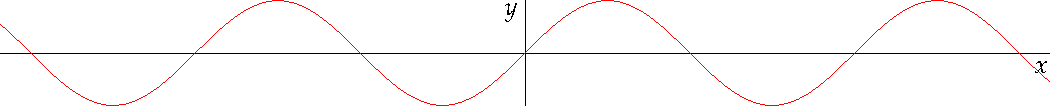
\includegraphics[width=\linewidth]{fg-tufte-wide-sine}%
  \caption[Example file fg-tufte-wide-sine.tex][2ex]
  {This graph shows $y = \sin x$ from about $x = [-10, 10]$.
  \emph{Notice that this figure takes up the full page width.}}%
  \label{fg-tufte-wide-sine}%
\end{figure*}


\vspace*{1ex} %% required to keep distance from full-width figure above.
\begin{algorithm-wide}[h]{1.55\textwidth}%  1.55\textwith expands to full width of figure above!!
\begin{algorithmic}[1]
\PROCEDURE{\CALL{newPivot.saw}{${\underline \varsigma}_{\omega_{s} -1},Walk_{\omega_{s} -1}$}}
\STATE $\mathbb{Z} \gets i = 1,2, \ldots ,L $ 
\STATE $\mathbb{Z}_p \gets permute(\mathbb{Z}) $ 
\STATE ${\cal N} ({\underline \varsigma}_{\omega_{s} -1}) \gets  \{{\underline \varsigma}_{\omega_{s} -1}^i | d({\underline \varsigma}_{\omega_{s} -1}, {\underline \varsigma}_{\omega_{s} -1}^i ) = 1, i \in \mathbb{Z}_p\}$ 
\STATE ${\cal N}_{saw} ({\underline \varsigma}_{\omega_{s} -1}) \gets  \{ {\cal N} ({\underline \varsigma}_{\omega -1}) |
                      {\underline \varsigma}_{\omega_{s} -1}^i \not\in  Walk_{\omega_{s} -1}\}$
   \IF {\strut  ${\cal N}_{saw}  ({\underline \varsigma}_{\omega_{s} -1}) \not= \emptyset$}  
        \STATE ${\underline \varsigma}_{\omega_{s}}\!:\!\Theta({\underline \varsigma}_{\omega_{s}}) \gets {\tt bestNeighbor}({\cal N}_{saw} ({\underline \varsigma}_{\omega_{s} -1}))$
        \STATE $Walk_{\omega_{s}} \gets Walk_{\omega_{s}-1} \cup \{{\underline \varsigma}_{\omega_{s}}\}$
        \STATE $\tau \gets \tau + |~{\cal N}_{saw} ({\underline \varsigma}_{\omega_{s} -1})~| $ 
        \COMMENT{update $cntProbe$}
   \ELSE[\textbf{deal with a trapped pivot}]
        \STATE $\beta = \beta + 1$ 
        \STATE ${\underline \varsigma}_{\omega_{s}}\!:\!\Theta({\underline \varsigma}_{\omega_{s}}) \gets {\tt coordInit}()$ 
        \COMMENT{re-initialize}
        \STATE $Walk_{\omega_{s}} \gets \{ {\underline \varsigma}_{\omega_{s}} \}$
        \STATE $\tau \gets \tau + 1 $ 
        \COMMENT{update $cntProbe$}
    \ENDIF
\STATE \textbf{return} $Walk_{\omega_{s}}\!:\!{\underline \varsigma}_{\omega_{s}}\!:\!\Theta({\underline \varsigma}_{\omega_{s}})$ 
\ENDPROCEDURE 
\end{algorithmic}
\caption[Algorithm file: alg-newPivot-wide.tex]{Procedure newPivot.saw -- using algorithm-wide environment.} 
\label{alg-newPivot-wide}
\end{algorithm-wide}

\newthought{Notably}, typesetting of the Algorithm~\ref{alg-newPivot-wide} results in excessive width, for better rendition 
of identical algorithm, see
Algorithm~\ref{alg-newPivot-normal} in the preceding page.

\lipsum[4]

\newthought{On the next page}, Algorithm~\ref{alg-global-search2-normal}
takes a full page at normal width. However, the version
in  Algorithm~\ref{alg-global-search2-wide} describes the same
algorithm, also on a full page, but in a wider, easier-to-read 
format.


\begin{algorithm}[!T]
\begin{footnotesize}
\begin{minipage}[!T]{0.99\linewidth}
\begin{algorithmic}[1]
\PROCEDURE{\CALL{lssOrel}{$\sigma_0, \Theta^{ub}_L, t_{lmt}, \omega_{lmt}$}}
\STATE {${\underline \varsigma}_0\!:\!\Theta({\underline \varsigma}_0) \gets {\tt coordInit}(\sigma_0)$}
\COMMENT{initial solution}
\STATE $\tau \gets 1 $ 
\COMMENT {initialize cntProbe}
\STATE ${\underline \varsigma^*}\!:\!\Theta({\underline \varsigma^*}) \gets {\underline \varsigma}_0\!:\!\Theta({\underline \varsigma}_0)$ 
\COMMENT{initial best solution} 
\STATE $isCens \gets 0$
\COMMENT{initialize $isCensored$}
\STATE $tgReached \gets 0$                                     
\COMMENT{initialize $targetReached$}
\STATE $\beta \gets 0$                                         
\COMMENT{initialize $cntTrapped$}
\STATE $\omega \gets 0$                                        
\COMMENT{initialize total number of steps}
\WHILE {{\bf true}}
  \STATE $\omega_{s}\!:\!{\underline \varsigma^*}\!:\!\Theta({\underline \varsigma^*}) \gets {\tt walk.saw}({\underline \varsigma}_{0}\!:\!\Theta({\underline \varsigma}_{0}),t_{lmt},\omega_{lmt})$ 
  \COMMENT{return a completed walk segment}
  \STATE $\omega \gets \omega + \omega_{s} $                   
  \COMMENT{update total number of steps}
  \IF{$\Theta({\underline \varsigma^*}) \leq \Theta^{ub}_L$}
    \IF {$\Theta({\underline \varsigma^*}) = \Theta^{ub}_L$}
      \STATE{$tgReached = 1$}                                  
      \COMMENT{upper-bound is reached}
    \ELSE
      \STATE $tgReached = 2$                                   
      \COMMENT{upper-bound is improved}
    \ENDIF
    \STATE {\bf{break}}
  \ENDIF
  \IF{$t \geq t_{lmt}$}
    \STATE $isCens \gets 1$                                    
    \COMMENT{return solution as ``censored''}
    \STATE {\bf{break}}
  \ENDIF
  \STATE ${\underline \varsigma}_0\!:\!\Theta({\underline \varsigma}_0) \gets {\tt coordInit}()$ 
  \COMMENT{initialize a new walk segment}
  \STATE $\tau \gets \tau + 1 $                               
  \COMMENT{update $cntProbe$}
  \STATE $\omega \gets \omega + 1 $                           
  \COMMENT{update total number of steps}
\ENDWHILE
\STATE $Table \gets (\sigma_0, {\underline \varsigma^*}, \Theta({\underline \varsigma^*}), \omega, \tau, t, isCens, tgReached)$
\ENDPROCEDURE
\end{algorithmic}
\end{minipage}

\vspace{0.2cm}
\begin{minipage}[!T]{0.49\linewidth}
\begin{algorithmic}[1]
\PROCEDURE{\CALL{walk.saw}{${\underline \varsigma}_{0}\!:\!\Theta({\underline \varsigma}_{0}),t_{lmt}, \omega_{lmt}$}}
\IF {$\Theta({\underline \varsigma}_{0}) \le \Theta({\underline \varsigma^*})$}
    \STATE ${\underline \varsigma^*}\!:\!\Theta({\underline \varsigma^*}) \gets {\underline \varsigma}_0\!:\!\Theta({\underline \varsigma}_0)$
    \COMMENT{new best solution}
\ENDIF
\STATE $\omega_{s} \gets 0$     
\COMMENT{walk segment length}                                   
\STATE $Walk_{0} \gets \{ {\underline \varsigma}_0 \}$
\COMMENT{new walk segment}
\WHILE {$\Theta({\underline \varsigma^*})  > \Theta^{ub}_L$ \textbf{and} $\omega_{s} < \omega_{lmt}$}
    \IF [timeout]{$t \geq t_{lmt}$}
        \STATE {\bf break}
    \ENDIF
    \STATE $\omega_{s}=\omega_{s}+1$
    \COMMENT{{\bf a new step!}}
    \STATE $Walk_{\omega_{s}}\!:\!{\underline \varsigma}_{\omega_{s}}\!:\!\Theta({\underline \varsigma}_{\omega_{s}}) \gets$
    \STATE { \hspace{0.5cm} $ \gets {\tt newPivot.saw}({\underline \varsigma}_{\omega_{s} - 1}, Walk_{\omega_{s} - 1})$}
     \IF { $\Theta({\underline \varsigma}_{\omega_{s}}) \le \Theta({\underline \varsigma^*})$} 
       \STATE ${\underline \varsigma^*}\!:\!\Theta({\underline \varsigma^*}) \gets {\underline \varsigma_{\omega_{s}}}\!:\!\Theta({\underline \varsigma}_{\omega_{s}})$
     \ENDIF
\ENDWHILE
\STATE {\bf return} $\omega_{s}\!:\!{\underline \varsigma^*}\!:\!\Theta({\underline \varsigma^*})$
\ENDPROCEDURE
\end{algorithmic}
\end{minipage}
\begin{minipage}[!T]{0.49\linewidth}
\label{fg_global_search_c}
\begin{algorithmic}[1]
\PROCEDURE{\CALL{newPivot.saw}{${\underline \varsigma}_{\omega_{s} -1},Walk_{\omega_{s} -1}$}}
\STATE $\mathbb{Z} \gets i = 1,2, \ldots ,L $ 
\STATE $\mathbb{Z}_p \gets permute(\mathbb{Z}) $ 
\STATE ${\cal N} ({\underline \varsigma}_{\omega_{s} -1}) \gets  \{{\underline \varsigma}_{\omega_{s} -1}^i | d({\underline \varsigma}_{\omega_{s} -1}, {\underline \varsigma}_{\omega_{s} -1}^i ) = 1, i \in \mathbb{Z}_p\}$ 
\STATE ${\cal N}_{saw} ({\underline \varsigma}_{\omega_{s} -1}) \gets  \{ {\cal N} ({\underline \varsigma}_{\omega -1}) |
                      {\underline \varsigma}_{\omega_{s} -1}^i \not\in  Walk_{\omega_{s} -1}\}$
   \IF {\strut  ${\cal N}_{saw}  ({\underline \varsigma}_{\omega_{s} -1}) \not= \emptyset$}  
        \STATE ${\underline \varsigma}_{\omega_{s}}\!:\!\Theta({\underline \varsigma}_{\omega_{s}}) \gets {\tt bestNeighbor}({\cal N}_{saw} ({\underline \varsigma}_{\omega_{s} -1}))$
        \STATE $Walk_{\omega_{s}} \gets Walk_{\omega_{s}-1} \cup \{{\underline \varsigma}_{\omega_{s}}\}$
        \STATE $\tau \gets \tau + |~{\cal N}_{saw} ({\underline \varsigma}_{\omega_{s} -1})~| $ 
        \COMMENT{update $cntProbe$}
   \ELSE[\textbf{deal with a trapped pivot}]
        \STATE $\beta = \beta + 1$ 
        \STATE ${\underline \varsigma}_{\omega_{s}}\!:\!\Theta({\underline \varsigma}_{\omega_{s}}) \gets {\tt coordInit}()$ 
        \COMMENT{re-initialize}
        \STATE $Walk_{\omega_{s}} \gets \{ {\underline \varsigma}_{\omega_{s}} \}$
        \STATE $\tau \gets \tau + 1 $ 
        \COMMENT{update $cntProbe$}
    \ENDIF
\STATE \textbf{return} $Walk_{\omega_{s}}\!:\!{\underline \varsigma}_{\omega_{s}}\!:\!\Theta({\underline \varsigma}_{\omega_{s}})$ 
\ENDPROCEDURE 
\end{algorithmic}
\end{minipage}
\caption[Algorithm file: alg-global-search2-normal.tex]{A fully instrumented version of solver \lssOrel\ -- normal width.} 
\label{alg-global-search2-normal}
\end{footnotesize}
\end{algorithm}

%\begin{Algorithm}[!T]{15cm}
\begin{algorithm-wide}[h]{1.5\textwidth}%  1.55\textwith expands to full width of widest figure
\begin{footnotesize}
\begin{minipage}[!T]{0.99\linewidth}
\begin{algorithmic}[1]
\PROCEDURE{\CALL{lssOrel}{$\sigma_0, \Theta^{ub}_L, t_{lmt}, \omega_{lmt}$}}
\STATE {${\underline \varsigma}_0\!:\!\Theta({\underline \varsigma}_0) \gets {\tt coordInit}(\sigma_0)$}
\COMMENT{initial solution}
\STATE $\tau \gets 1 $ 
\COMMENT {initialize cntProbe}
\STATE ${\underline \varsigma^*}\!:\!\Theta({\underline \varsigma^*}) \gets {\underline \varsigma}_0\!:\!\Theta({\underline \varsigma}_0)$ 
\COMMENT{initial best solution} 
\STATE $isCens \gets 0$
\COMMENT{initialize $isCensored$}
\STATE $tgReached \gets 0$                                     
\COMMENT{initialize $targetReached$}
\STATE $\beta \gets 0$                                         
\COMMENT{initialize $cntTrapped$}
\STATE $\omega \gets 0$                                        
\COMMENT{initialize total number of steps}
\WHILE {{\bf true}}
  \STATE $\omega_{s}\!:\!{\underline \varsigma^*}\!:\!\Theta({\underline \varsigma^*}) \gets {\tt walk.saw}({\underline \varsigma}_{0}\!:\!\Theta({\underline \varsigma}_{0}),t_{lmt},\omega_{lmt})$ 
  \COMMENT{return a completed walk segment}
  \STATE $\omega \gets \omega + \omega_{s} $                   
  \COMMENT{update total number of steps}
  \IF{$\Theta({\underline \varsigma^*}) \leq \Theta^{ub}_L$}
    \IF {$\Theta({\underline \varsigma^*}) = \Theta^{ub}_L$}
      \STATE{$tgReached = 1$}                                  
      \COMMENT{upper-bound is reached}
    \ELSE
      \STATE $tgReached = 2$                                   
      \COMMENT{upper-bound is improved}
    \ENDIF
    \STATE {\bf{break}}
  \ENDIF
  \IF{$t \geq t_{lmt}$}
    \STATE $isCens \gets 1$                                    
    \COMMENT{return solution as ``censored''}
    \STATE {\bf{break}}
  \ENDIF
  \STATE ${\underline \varsigma}_0\!:\!\Theta({\underline \varsigma}_0) \gets {\tt coordInit}()$ 
  \COMMENT{initialize a new walk segment}
  \STATE $\tau \gets \tau + 1 $                               
  \COMMENT{update $cntProbe$}
  \STATE $\omega \gets \omega + 1 $                           
  \COMMENT{update total number of steps}
\ENDWHILE
\STATE $Table \gets (\sigma_0, {\underline \varsigma^*}, \Theta({\underline \varsigma^*}), \omega, \tau, t, isCens, tgReached)$
\ENDPROCEDURE
\end{algorithmic}
\end{minipage}

\vspace{0.2cm}
\begin{minipage}[!T]{0.49\linewidth}
\begin{algorithmic}[1]
\PROCEDURE{\CALL{walk.saw}{${\underline \varsigma}_{0}\!:\!\Theta({\underline \varsigma}_{0}),t_{lmt}, \omega_{lmt}$}}
\IF {$\Theta({\underline \varsigma}_{0}) \le \Theta({\underline \varsigma^*})$}
    \STATE ${\underline \varsigma^*}\!:\!\Theta({\underline \varsigma^*}) \gets {\underline \varsigma}_0\!:\!\Theta({\underline \varsigma}_0)$
    \COMMENT{new best solution}
\ENDIF
\STATE $\omega_{s} \gets 0$     
\COMMENT{walk segment length}                                   
\STATE $Walk_{0} \gets \{ {\underline \varsigma}_0 \}$
\COMMENT{new walk segment}
\WHILE {$\Theta({\underline \varsigma^*})  > \Theta^{ub}_L$ \textbf{and} $\omega_{s} < \omega_{lmt}$}
    \IF [timeout]{$t \geq t_{lmt}$}
        \STATE {\bf break}
    \ENDIF
    \STATE $\omega_{s}=\omega_{s}+1$
    \COMMENT{{\bf a new step!}}
    \STATE $Walk_{\omega_{s}}\!:\!{\underline \varsigma}_{\omega_{s}}\!:\!\Theta({\underline \varsigma}_{\omega_{s}}) \gets$
    \STATE { \hspace{0.5cm} $ \gets {\tt newPivot.saw}({\underline \varsigma}_{\omega_{s} - 1}, Walk_{\omega_{s} - 1})$}
     \IF { $\Theta({\underline \varsigma}_{\omega_{s}}) \le \Theta({\underline \varsigma^*})$} 
       \STATE ${\underline \varsigma^*}\!:\!\Theta({\underline \varsigma^*}) \gets {\underline \varsigma_{\omega_{s}}}\!:\!\Theta({\underline \varsigma}_{\omega_{s}})$
     \ENDIF
\ENDWHILE
\STATE {\bf return} $\omega_{s}\!:\!{\underline \varsigma^*}\!:\!\Theta({\underline \varsigma^*})$
\ENDPROCEDURE
\end{algorithmic}
\end{minipage}
\begin{minipage}[!T]{0.49\linewidth}
\label{alg-global-search2-wide-c}
\begin{algorithmic}[1]
\PROCEDURE{\CALL{newPivot.saw}{${\underline \varsigma}_{\omega_{s} -1},Walk_{\omega_{s} -1}$}}
\STATE $\mathbb{Z} \gets i = 1,2, \ldots ,L $ 
\STATE $\mathbb{Z}_p \gets permute(\mathbb{Z}) $ 
\STATE ${\cal N} ({\underline \varsigma}_{\omega_{s} -1}) \gets  \{{\underline \varsigma}_{\omega_{s} -1}^i | d({\underline \varsigma}_{\omega_{s} -1}, {\underline \varsigma}_{\omega_{s} -1}^i ) = 1, i \in \mathbb{Z}_p\}$ 
\STATE ${\cal N}_{saw} ({\underline \varsigma}_{\omega_{s} -1}) \gets  \{ {\cal N} ({\underline \varsigma}_{\omega -1}) |
                      {\underline \varsigma}_{\omega_{s} -1}^i \not\in  Walk_{\omega_{s} -1}\}$
   \IF {\strut  ${\cal N}_{saw}  ({\underline \varsigma}_{\omega_{s} -1}) \not= \emptyset$}  
        \STATE ${\underline \varsigma}_{\omega_{s}}\!:\!\Theta({\underline \varsigma}_{\omega_{s}}) \gets {\tt bestNeighbor}({\cal N}_{saw} ({\underline \varsigma}_{\omega_{s} -1}))$
        \STATE $Walk_{\omega_{s}} \gets Walk_{\omega_{s}-1} \cup \{{\underline \varsigma}_{\omega_{s}}\}$
        \STATE $\tau \gets \tau + |~{\cal N}_{saw} ({\underline \varsigma}_{\omega_{s} -1})~| $ 
        \COMMENT{update $cntProbe$}
   \ELSE[\textbf{deal with a trapped pivot}]
        \STATE $\beta = \beta + 1$ 
        \STATE ${\underline \varsigma}_{\omega_{s}}\!:\!\Theta({\underline \varsigma}_{\omega_{s}}) \gets {\tt coordInit}()$ 
        \COMMENT{re-initialize}
        \STATE $Walk_{\omega_{s}} \gets \{ {\underline \varsigma}_{\omega_{s}} \}$
        \STATE $\tau \gets \tau + 1 $ 
        \COMMENT{update $cntProbe$}
    \ENDIF
\STATE \textbf{return} $Walk_{\omega_{s}}\!:\!{\underline \varsigma}_{\omega_{s}}\!:\!\Theta({\underline \varsigma}_{\omega_{s}})$ 
\ENDPROCEDURE 
\end{algorithmic}
\end{minipage}
\caption[Algorithm file: alg-global-search2-wide.tex]{A fully instrumented version of solver \lssOrel\ -- using algorithm-wide environment.} 
\label{alg-global-search2-wide}
\end{footnotesize}
\end{algorithm-wide}

\clearpage
%\begin{algorithm-wide}[h]{15cm}
\begin{algorithm-wide}[!t]{1.5\textwidth}%  1.55\textwith expands to full width of widest figure
\begin{footnotesize}
\begin{minipage}[!T]{0.52\linewidth}
\centering
\begin{algorithmic}[1]
\PROCEDURE{\CALL{lssMAts}{$\Theta^{ub}_L, t_{lmt}$}}
\FOR{$i\gets 1$ {\bf to} $popsize$} \label{alg_lssMAts_For1}
    \STATE $pop_i\gets$ \CALL{RandomBinarySequence}{$L$}
    \STATE \CALL{Evaluate}{$pop_i$}
\ENDFOR \label{alg_lssMAts_For2}
\STATE \colorbox{Gray}{\valueBest $\gets \CALL{ValueBest}{pop}$}
\WHILE {\colorbox{Gray}{ $t < t_{lmt}$ {\bf ~and~}  \valueBest $\,>\,$ \valueTarget} }
    \FOR{$i=1$ {\bf to} $\mathit{offsize}$}     
        \IF {recombination is performed ($p_X$)} \label{alg_lssMAts_Rec1}
            \STATE $parent_1 \gets $\CALL{Select}{$pop$}
            \STATE $parent_2 \gets $\CALL{Select}{$pop$}
            \STATE $\mathit{offspring_i}\gets$\CALL{Recombine}{$parent_1, parent_2$}
        \ELSE
            \STATE $\mathit{offspring}_i \gets $\CALL{Select}{$pop$}
        \ENDIF \label{alg_lssMAts_Rec2}
        \IF {mutation is performed ($p_m$)} \label{alg_lssMAts_Mut1}
            \STATE $\mathit{offspring}_i \gets $\CALL{Mutate}{$\mathit{offspring}_i$}
        \ENDIF \label{alg_lssMAts_Mut2}
        \STATE $\mathit{offspring}_i \gets$\CALL{TabuSearch}{$\mathit{offspring}_i$}
        \STATE \CALL{Evaluate}{$\mathit{offspring}_i$}
    \ENDFOR
    \STATE $pop \gets$\CALL{Replace}{$pop$, $\mathit{offspring}$} \label{alg_lssMAts_Sel}
    \STATE \colorbox{Gray}{\valueBest $\gets \CALL{ValueBest}{pop}$}
\ENDWHILE
\ENDPROCEDURE 
\end{algorithmic}
\end{minipage}
\begin{minipage}[!T]{0.52\linewidth}
% {\small	
% % The procedure \lssMAts\ on the left is an instrumented versions of the 
% % \labs\ solver named as $MA_{TS}$
% % in~\cite{Lib-OPUS-labs-2009-ASC-Gallardo-memetic}.
% % Settings of all parameters,
% % used also in our experiments, are described
% % in~\cite{Lib-OPUS-labs-2009-ASC-Gallardo-memetic}.
% % See a concise reprise below.
\par\vspace*{1ex}
\begin{tabular}{l l}
 {\bf setting} & {\bf value} \\
 \hline
 population size: & 100 \\
 mutation probability: & $2/(L+1)$ \\
 crossover probability: & 0.9 \\
 tournament selection size: & 2 \\
 crossover: & uniform \\
 tabu search walk length: & a random choice  \\
 ~~              &  from the range\\
 ~~              & {\small [$\frac{L}{2}, \frac{3 L}{2}$]}\\
 ~~              & ~~
\end{tabular}
%\centering
\begin{algorithmic}[1]
\PROCEDURE{\CALL{lssRRts}{$\Theta^{ub}_L, t_{lmt}$}}
\STATE $pop_1\gets$ \CALL{RandomBinarySequence}{$L$}
\STATE \CALL{Evaluate}{$pop_1$}
\STATE \colorbox{Gray} {\valueBest $\gets \CALL{ValueBest}{pop}$}
\WHILE {\colorbox{Gray}{ $t < t_{lmt}$ {\bf ~and~}  \valueBest $\,>\,$ \valueTarget} }
        \STATE $\mathit{pop_1} \gets $\CALL{RandomBinarySequence}{$L$}
        \STATE $\mathit{pop_1} \gets $\CALL{TabuSearch}{$\mathit{pop_1}$}
        \STATE \CALL{Evaluate}{$\mathit{pop_1}$}
        \STATE \colorbox{Gray}{\valueBest $\gets \CALL{ValueBest}{pop}$}
\ENDWHILE
\ENDPROCEDURE 
\end{algorithmic}
\vspace{2cm}
\end{minipage}
\caption[Algorithm file: alg-lssMAts-lssRRts-wide.tex]{\lssMAts\ and \lssRRts\ algorithms -- using algorithm-wide environment.} 
\label{alg-lssMAts-lssRRts-wide}
\end{footnotesize}
\end{algorithm-wide}

\newthought{On this page}, Algorithm~\ref{alg-lssMAts-lssRRts-wide}
is placed at the top of the page with the [!t] option.
\lipsum[4]
\lipsum[1]

\newthought{Here is} a simple in-line Algorithm description we can include, with some restrictions, in a margin note as well.
\begin{algorithm}
\begin{algorithmic}[1]
\PROCEDURE{\CALL{lssRRts}{$\Theta^{ub}_L, t_{lmt}$}}
\STATE $pop_1\gets$ \CALL{RandomBinarySequence}{$L$}
\STATE \CALL{Evaluate}{$pop_1$}
\STATE \colorbox{Gray} {\valueBest $\gets \CALL{ValueBest}{pop}$}
\WHILE {\colorbox{Gray}{ $t < t_{lmt}$ {\bf ~and~}  \valueBest $\,>\,$ \valueTarget} }
        \STATE $\mathit{pop_1} \gets $\CALL{RandomBinarySequence}{$L$}
        \STATE $\mathit{pop_1} \gets $\CALL{TabuSearch}{$\mathit{pop_1}$}
        \STATE \CALL{Evaluate}{$\mathit{pop_1}$}
        \STATE \colorbox{Gray}{\valueBest $\gets \CALL{ValueBest}{pop}$}
\ENDWHILE
\ENDPROCEDURE 
\end{algorithmic}
\caption{Pseudo code for \lssRRts\ -- in-line version}.
\end{algorithm}

\newthought{Here is a margin note} for a 
pseudo-code that describes a simple procedure\marginnote[-6ex]{
%\begin{algorithm} %%%% does NOT work with \marginnote
\begin{algorithmic}[1]
\PROCEDURE{\CALL{lssRRts}{$\Theta^{ub}_L, t_{lmt}$}}
\STATE $pop_1\gets$ \CALL{RandBinSeq}{$L$}
\STATE \CALL{Evaluate}{$pop_1$}
\STATE \colorbox{Gray} {\valueBest $\gets \CALL{ValueBest}{pop}$}
\WHILE {\colorbox{Gray}{ $t < t_{lmt}$ {\bf ~and~}  \valueBest $\,>\,$ \valueTarget} }
        \STATE $\mathit{pop_1} \gets $\CALL{RandBinSeq}{$L$}
        \STATE $\mathit{pop_1} \gets $\CALL{TabuSearch}{$\mathit{pop_1}$}
        \STATE \CALL{Evaluate}{$\mathit{pop_1}$}
        \STATE \colorbox{Gray}{\valueBest $\gets \CALL{ValueBest}{pop}$}
\ENDWHILE
\ENDPROCEDURE 
\end{algorithmic}
%\caption{Pseudo code for \lssRRts}.
%\end{algorithm}
}. NOTE: we cannot use the \verb+\algorithm+ and \verb+\caption+ environment 
under  \verb+\marginnote+.

\lipsum[4]


 